\subsection{TPC1 Tracking Efficiency}
\label{sec:Systematics_TPC1tracking}

When calculating the \p0d tracking and matching efficiency in Section \ref{sec:Systematics_Efficiency}, we used a selection of tracks which had been reconstructed in TPC1. In this section, we now evaluate the systematic uncertainty arising from the efficiency of reconstrucing a track in TPC1 using sub-detector reconstruction only. 
The work for this was completed by Anthony Hillairet and the tracker group. The technique uses a selection of events with reconstructed tracks in the \p0d and TPC2 and looks for the fraction of time where there is also a reconstructed track in TPC1. Further details can be found in the draft T2K technical note detailing tracking efficiency in the ND280 Tracker (T2K-TN-075). The efficiency is expected to be very high and the systematic uncertainty very low so we linearly add the central \textit{in}-efficiency ratio value with the error to calculate the final systematic. The results are binned in muon track candidate momentum.% (0-2 GeV, 2-5 GeV and 5-20 GeV).

\begin{figure}[here]
\centering
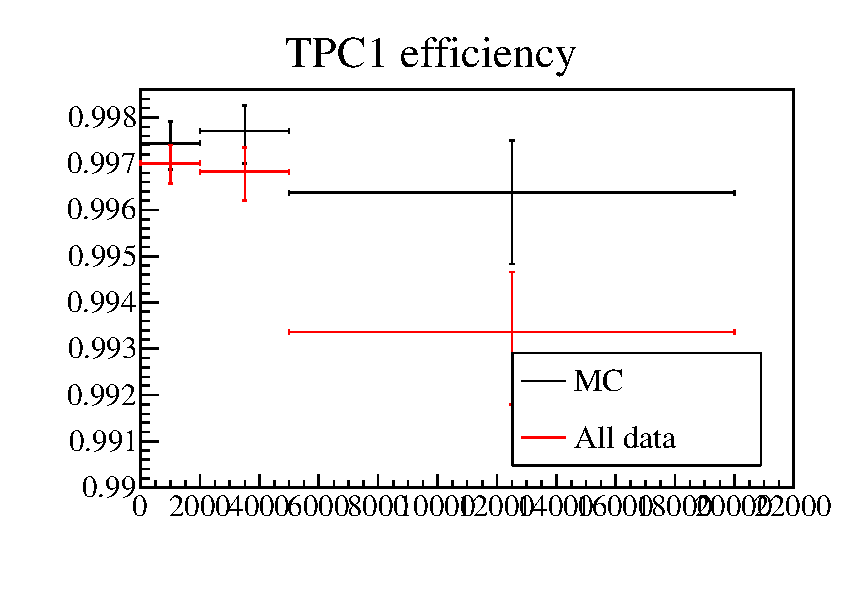
\includegraphics[width=4in]{Figures/TrkFdEf_TPC1_RajsBins.eps}
\caption{TPC1 Track Finding Efficiency vs. muon momentum. Black (Red) shows MC (Data). The plot is zero suppressed.}
\label{fig:tpc1eff}
\end{figure}

\begin{table}[here]
\caption{TPC1 Track finding efficiencies and ratios of efficiency for MC and Data. Errors are also shown. All numbers are percentages.}
\label{tab:tpc1eff}
\centering
\begin{tabular}{cccccc}\toprule
& MC & Data & Ratio & \% Data Events& \% Data Events \\
& MC & Data & Ratio & \% Water-in & \% Water-Out \\ \midrule
0 - 2 GeV & $99.74 \pm 0.05 \%$ & $99.70 \pm 0.04 \%$ & $99.96 \pm 0.07 \%$ & 57.1 \% & 57.3 \% \\
2 - 5 GeV & $99.77 \pm 0.06 \%$ & $99.68 \pm 0.06 \%$ & $99.91 \pm 0.09 \%$ & 31.5 \% & 25.1 \% \\
5 - 20 GeV & $99.64 \pm 0.14 \%$ & $99.34 \pm 0.14 \%$ & $99.70 \pm 0.20 \%$ & 11.4 \% & 8.1 \%\\
\bottomrule
\end{tabular}
\end{table}

The TPC1 efficiency results are shown in Table \ref{tab:tpc1eff} and Figure \ref{fig:tpc1eff}. Linearly adding the inefficiency ratio and error, 
the TPC study obtains very small uncertainties of 0.1\%, 0.2\% and 0.5\% 
for momentum bins 0-2 GeV, 2-5 GeV and 5+ GeV respectively. 
These uncerainties are then weight-average with the percentage 
of selected events in each momentum bin for each run type. 
The systematic yielded by this study for a single momentum bin is $0.18 \%$ for water-in and $0.15 \%$ for water-out. 
As expected, the overall effect from tracking inefficiencies 
in the TPC is extremely small.
